% !TEX encoding = UTF-8 Unicode
\documentclass[12pt,a4paper]{article}

% Use some typical packages
\usepackage{epsfig,colordvi,subfigure,pdflscape,amssymb,url}
\usepackage{amsmath}
\usepackage{graphicx}

% Modify the page setup
\setlength{\topmargin}{-1.0in}
\setlength{\oddsidemargin}{0.in}
\setlength{\evensidemargin}{0.in}
\setlength{\textheight}{9.5 in}
\setlength{\textwidth}{6.3 in}

% Set some new commands
\renewcommand{\baselinestretch}{1.5}
\newcommand{\cl}{\centerline}

% Chinese characters
\usepackage{CJKutf8}
\newcommand{\cntext}[1]{\begin{CJK*}{UTF8}{bkai}#1\end{CJK*}}


% Begin the document
\begin{document}

% Title
\cl{\bf \Large Computational Physics}
\cl{\bf \large Homework \#1}
\cl{\bf \small 2024.02.20}
\cl{\small Name: Your Name}


% Start enumerating 

\begin{enumerate}

% Problem 1
\item Your solution for problem 1.  You could type mathematical equations easily with Latex. Equation~\ref{eq1} is a demo equation.

	% insert a equational
	\begin{equation} \label{eq1}
	F = \frac{G m_1 m_2}{r^2},
	\end{equation}


% Problem 2
\item Your solution for problem 2. You could include figures from your code. Figure~\ref{fig1} is xxx.

	% insert a figure
	\begin{figure}[h] 
		\begin{center}
		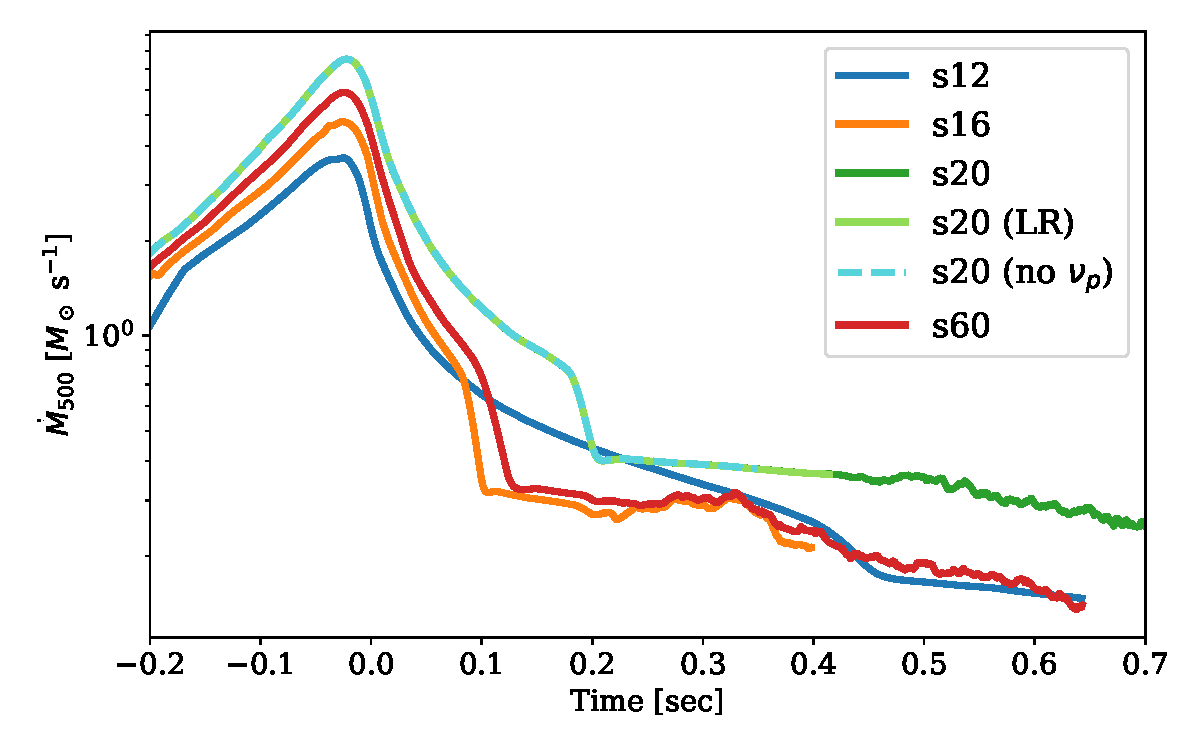
\includegraphics[scale=0.6]{fig_example.pdf} 
		\caption{This is a figure caption.  \label{fig1}}
		\end{center}
	\end{figure}

% Problem 3
\item Latex \cntext{也支援中文輸入。}
 
 
 % End of enumerating
\end{enumerate}

% End of document
\end{document}





